\section{Motivation}
\begin{frame}[t]{Motivation}
    \vskip-0.2cm
    \textbf{Increasing number of critical applications in Cloud}
	\vskip0.5cm
		\textbf{Intent to compromise:}
	\begin{itemize}
		\setlength{\wideitemsep}{2pt}
		\item Confidentiality
		\item Integrity
		\item Availability
	\end{itemize}
	\vspace{0.5cm}
	\textbf{Intrusion:}
	\begin{itemize}
		\setlength{\wideitemsep}{2pt}
		\item Intentional vulnerability exploitation
		\item Malicious fault
	\end{itemize}

	\vspace{0.5cm}
	Recover the application \textbf{integrity} to prevent \textbf{losses}

	\note{
	As aplicações web estão expostas a um ambiente não confiável em que as aplicações e os sistemas através dos quais estas são disponibilizados, sofrem ataques constantemente. Os ataques visam explorar vulnerabilidades para comprometer a confidencialidade, integridade e disponibilidade da aplicação. Se bem sucedido, o ataque provoca uma falta maliciosa.

	Importa relembrar que a disponibilidade do aplicação depende também da sua integridade. Se os dados corrompidos forem expostos aos utilizadores, ocorre um erro, e a aplicação falha, ficando indesponível. Uma aplicação indisponível e/ou com os dados corrompidos não só é inútil como também pode causar enormes prejuízos quer aos providers pela quebra do service level agreement, SLA, quer aos clientes que dependem da aplicação.}
\end{frame}

%%%%%%%%%%
% 01:45
%%%%%%%%%%%%%

%-------------------------------------------------------------------
\begin{frame}[t]{Motivation}
	\begin{center}
		\begin{figure}
		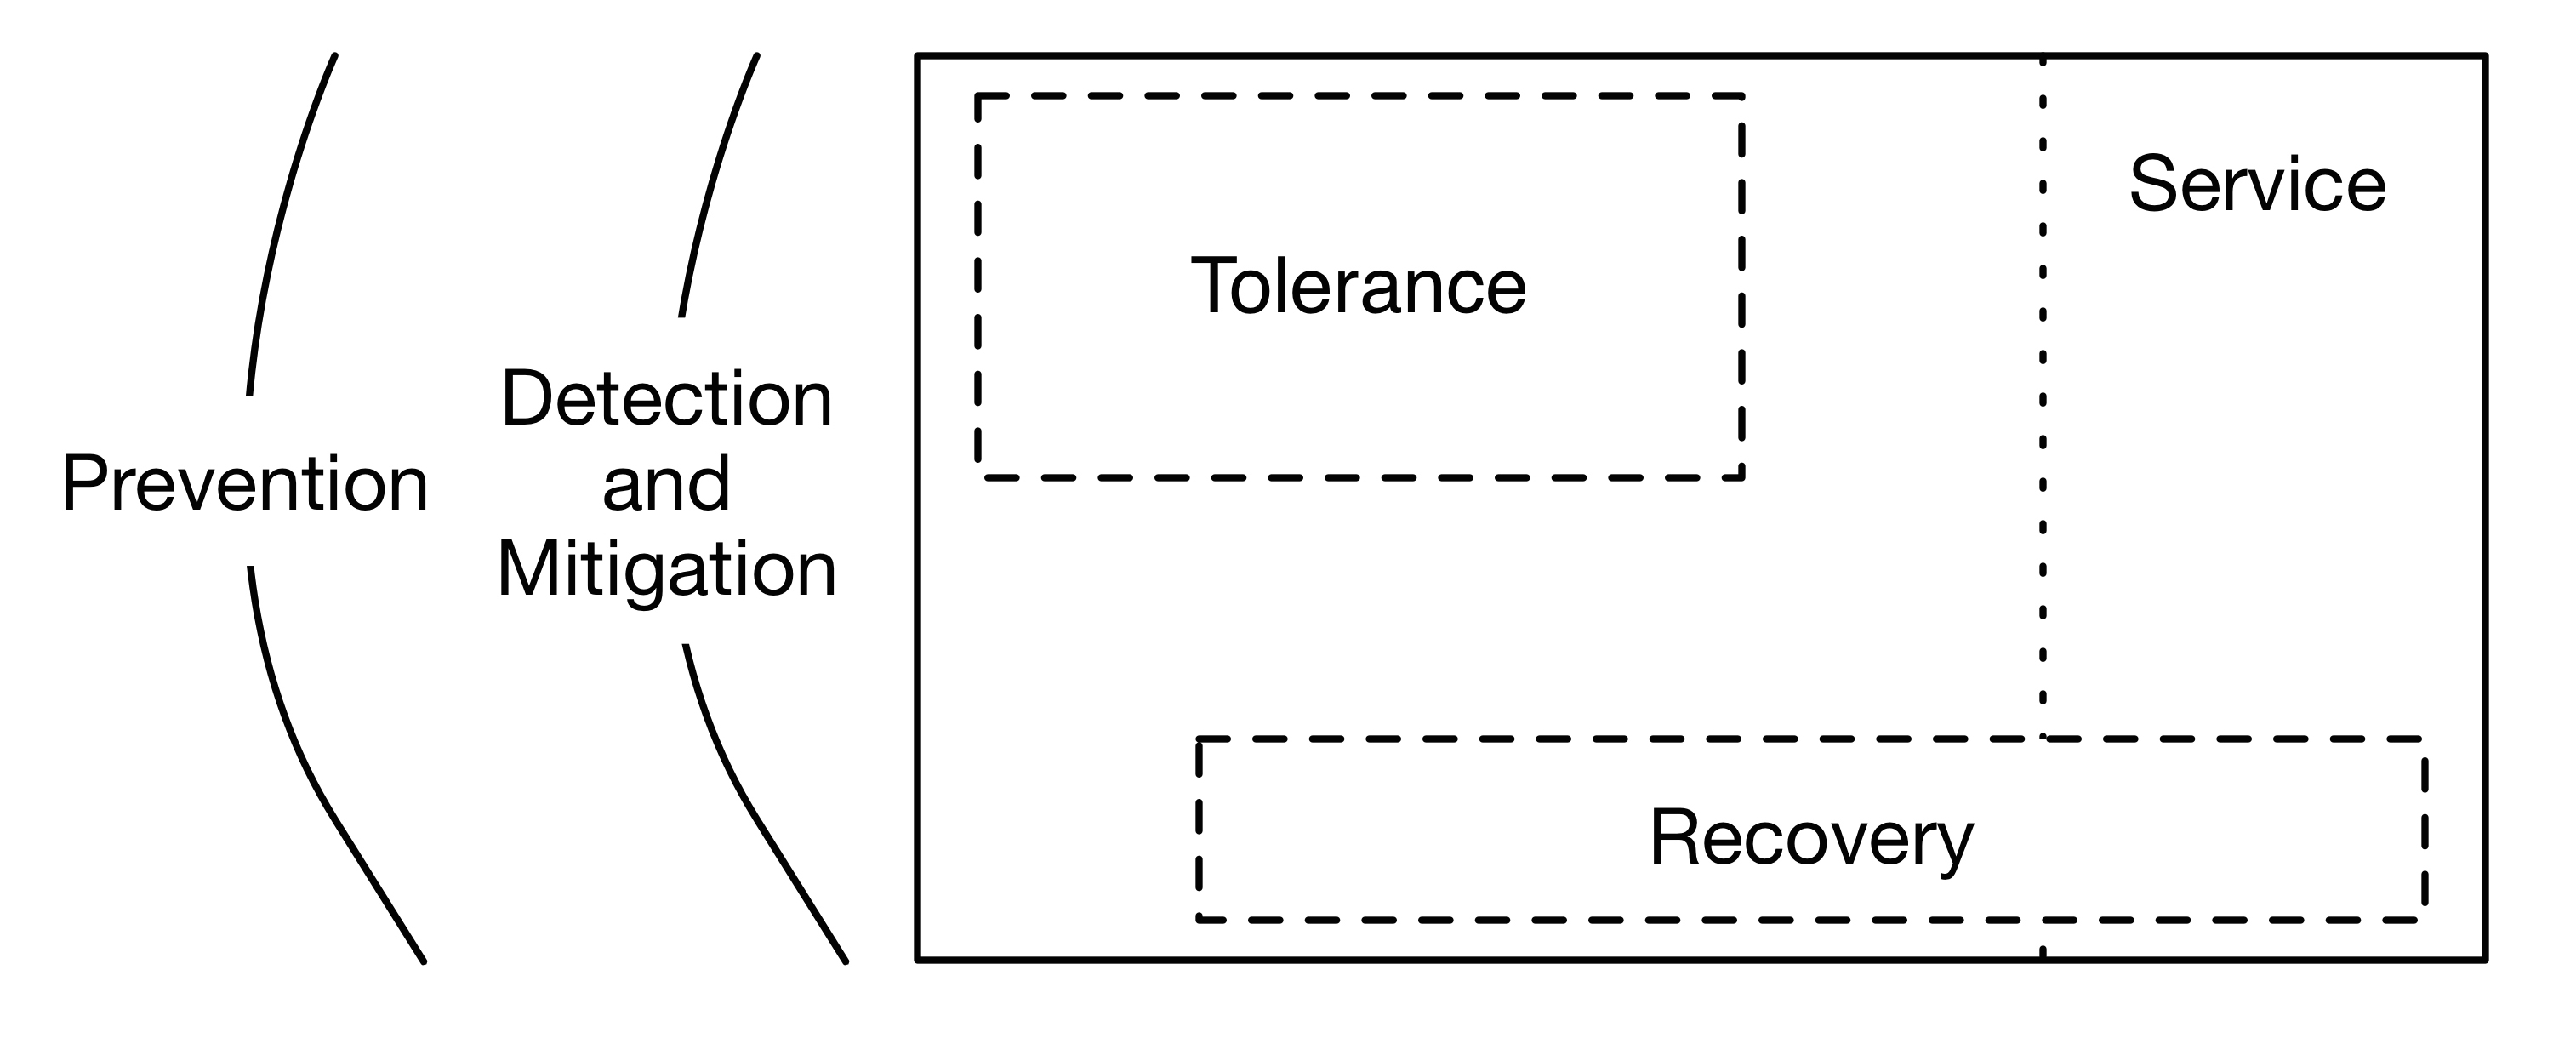
\includegraphics[width=0.8\textwidth]{img/ie0}
	 \end{figure}
	\end{center}
	\note{Para evitar perdas, as aplicações são protegidas por várias linhas de defesa: a prevenção, que tenta evitar ataques criem faltas no sistema. Depois, os mecanismos de detecção e tolerancia que tentam ocultar as faltas que ocorrem e por ultimo os mecanismos de recuperação que tentam recuperar dos erros e falhas.
	}
\end{frame}

%%%%%%%%%%
% 02:20
%%%%%%%%%%%%%

%-------------------------------------------------------------------
\begin{frame}[t]{Motivation}
	\vskip-0.5cm
	\begin{itemize}
		\setlength{\wideitemsep}{0.3cm}
		\item Software flaws
		\item New attack methods
		\item Configuration and usage mistakes (malicious or accidental)
		\item Legitimate requests
	\end{itemize}

	\begin{center}
			\begin{figure}
			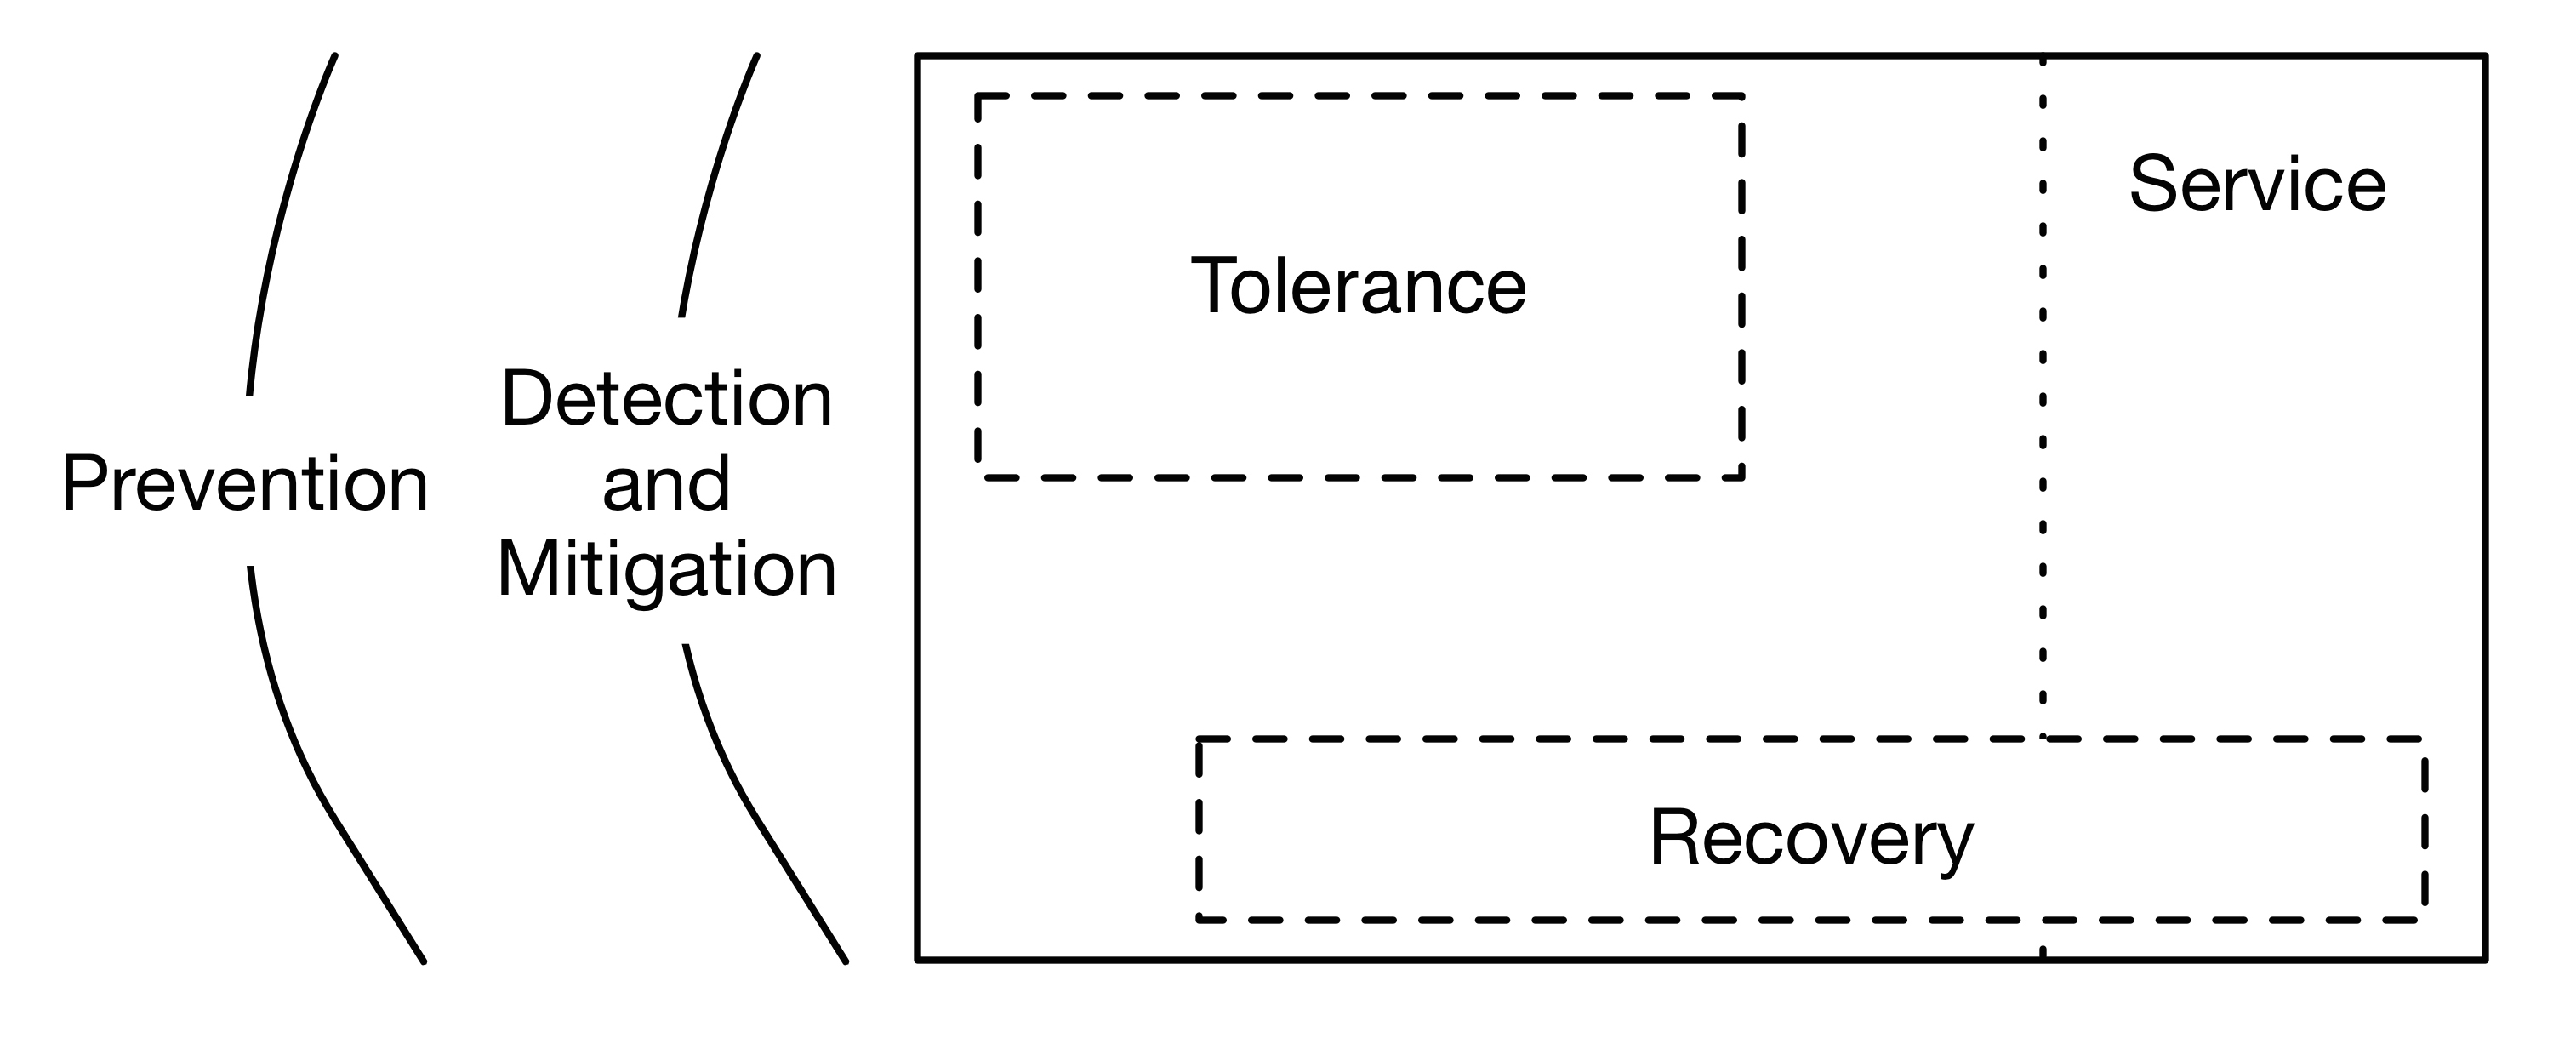
\includegraphics[width=0.7\textwidth]{img/ie0}
		 \end{figure}
	\end{center}
	\note{
	No entanto estes mecanismos são penetrados por ataques devido a novas vulnerabilidades no software e a novos métodos de ataque. Além disso, os administradores e utilizadores podem cometer erros acidentalmente ou maliciosamente na configuração ou utilizacação do sistema e, através de pedidos que são legitimos, corromper os dados da aplicação.
	Neste caso, além dos mecanismos de prevenção e detecção serem ultrapassados, os mecanismos de tolerancia vão replicar os dados corrompidos afectando todas as réplicas porque se tratam de pedidos legitimos e não de mensagens bizantinas.	      
	}
\end{frame}

%%%%%%%%%%
% 02:45
%%%%%%%%%%%%%
%-------------------------------------------------------------------
	
\begin{frame}[c]{Motivation}
	\begin{center}
	{\Large \textbf{Intrusions and failures happen!}} 
	\vspace{20pt}
		\begin{figure}
			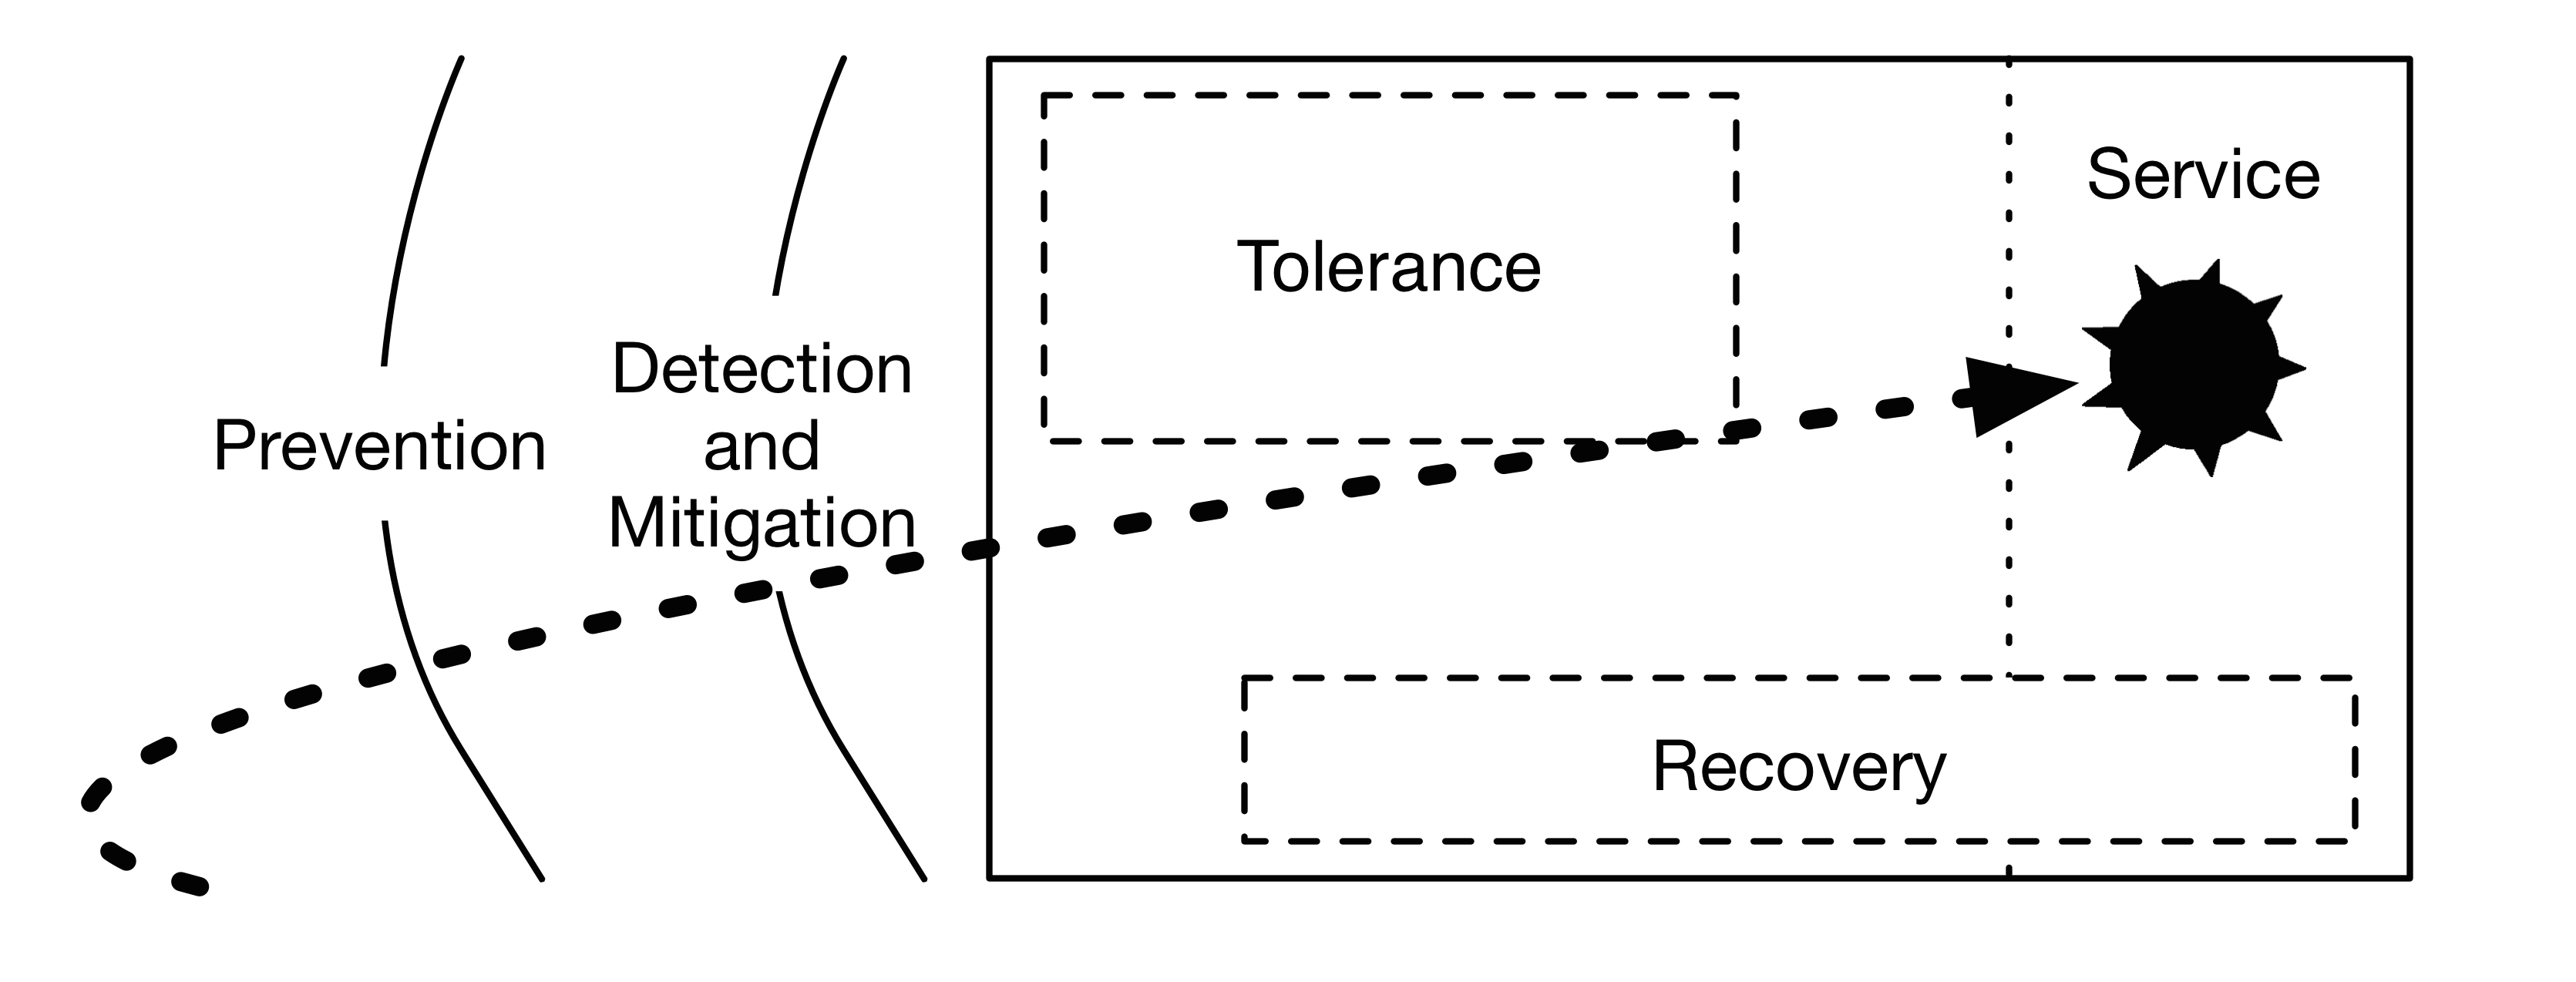
\includegraphics[width=0.8\textwidth]{img/ie4}
		\end{figure}	
	\end{center}
	\note{
	Como o nosso exemplo simples provou, as barreiras de segurança podem ser ultrapassadas. Haveriam muitos outros exemplos possíveis mas este em particular não só é frequente como também pode ser um simples erro do utilizador.
	Por isso, as intrusões podem acontecer.
	}
\end{frame}